%!TEX root = /Users/audrey/Dropbox/PhD/MOMAB/ArXiv/Latex/paper.tex

\section{Experiments}
\label{sec:experiments}

Given that the preference function is known a priori, one might be tempted to formalize the problem under the \emph{traditional}, single-objective, bandits setting. This would correspond to optimizing over the expected value of the preference function, $\Esp[f(\bsz(t)) | a(t) =a]$, instead of $f(\bsmu_a)$. In the following experiments, we compare the performance of the TS algorithm from MVN priors (Alg.~\ref{alg:mvn_ts}) in the multi-objective bandits scheme (Alg.~\ref{alg:mobandits}) with the one-dimensional TS from Gaussian priors~\cite{Agrawal2013} applied to the multi-objective bandits problem formalized under the traditional bandits setting (Alg.~\ref{alg:gaussian_ts}).

\begin{algorithm}[t]
    \begin{algorithmic}[1]
        \FORALL{episode $t \geq 1$}
            \FORALL{action $a \in \cA$}
                \STATE sample $\theta_a(t) = \Normal \big( \frac{N_a(T) \hat \mu_a(t)}{N_a(t) + 1}, \frac{1}{N_a(t) + 1} \big)$
            \ENDFOR
            \STATE play $a(t) = \argmax_{a \in \cA} \theta_a(t)$ and observe $f(\bsz(t))$
        \ENDFOR
    \end{algorithmic}
    \caption{Thompson sampling from Gaussian priors~\cite{Agrawal2013}}
\label{alg:gaussian_ts}
\end{algorithm}

We randomly generate a 10-action setting with $d = 2$ objectives, such that the objective space is $\cX = [0, 1]^2$. We consider settings where outcomes are sampled from multivariate normal distributions with covariance
$
    \bsSigma_a =
        \begin{bmatrix}
            0.10 & 0.05 \\
            0.05 & 0.10
        \end{bmatrix}
$ for all $a \in \cA$ and from multi-Bernoulli distributions. A sample $\bsz \sim \Bern_d(\bsmu)$ from a $d$-dimensional multi-Bernoulli distribution with mean $\bsmu$ is such that $z_i \sim \Bern(\mu_i)$. Experiments are conducted using the linear preference function
\begin{align*}
    f(\bsx) = 0.4 x_1 + 0.6 x_2, \quad \bsx \in \cX,
\end{align*}
and the $\epsilon$-constraint preference function
\begin{align*}
    f(\bsx) = \bigg\{
        \begin{array}{ll}
            x_2 & \quad \text{if} \quad x_1 \geq 0.5 \\
            0 & \quad \text{otherwise}
        \end{array}, \quad \bsx \in \cX.
\end{align*}
Tab.~\ref{tab:experiments:setting} gives the expected outcomes for all actions along with the associated preference value and gap given the preference function. Fig.~\ref{fig:experiments:setting} shows the expected outcomes and illustrates the preference function. We observe that the optimal action is different for the two preference functions. Each experiment is conducted over \num[group-separator={,}]{10000} episodes and repeated 100 times. Repetitions have been made such that the noise $\bsxi(t)$ is the same for all tested approaches on \emph{the same repetition}. Therefore we can compare the performance of different approaches on the same repetition. The goal is to minimize the cumulative regret (Eq.~\ref{eqn:regret}).

\begin{table}[t]
    \centering
    \caption{Expected outcomes with preference values and gap for both preference functions. The expected outcome for the optimal action is shown in bold.}
    \begin{tabular}{ccccc}
        \hline
        $\bsmu_a$ & \multicolumn{2}{c}{$f(\bsmu_a)$} & \multicolumn{2}{c}{$\Delta_a$} \\
        & Linear & $\epsilon$-constraint & Linear & $\epsilon$-constraint \\
        \hline
        $(0.56, 0.46)$ & 0.50 & 0.46 & 0.17 & 0.26 \\
        $(0.75, 0.26)$ & 0.46 & 0.26 & 0.21 & 0.46 \\
        $(0.34, 0.79)$ & 0.61 & 0.00 & 0.06 & 0.72 \\
        $(0.67, 0.50)$ & 0.56 & 0.50 & 0.11 & 0.22 \\
        $(0.70, 0.42)$ & 0.54 & 0.42 & 0.13 & 0.29 \\
        $(0.54, 0.72)$ & 0.65 & \textbf{0.72} & 0.02 & 0.00 \\
        $(0.49, 0.62)$ & 0.57 & 0.00 & 0.10 & 0.72 \\
        $(0.13, 0.84)$ & 0.56 & 0.00 & 0.11 & 0.72 \\
        $(0.78, 0.60)$ & \textbf{0.67} & 0.60 & 0.00 & 0.12 \\
        $(0.63, 0.44)$ & 0.51 & 0.44 & 0.16 & 0.28 \\
        \hline
    \end{tabular}
\label{tab:experiments:setting}
\end{table}

\begin{figure}[t]
    \centering
    \begin{subfigure}[b]{0.41\textwidth}
        \centering
        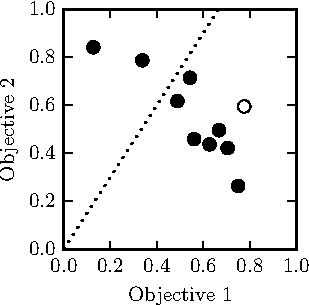
\includegraphics[scale=0.75]{linear}
        \caption{Linear with $\alpha_1 = 0.4$, $\alpha_2 = 0.6$}
        \label{fig:experiments:setting:linear}
    \end{subfigure}
    \qquad
    \begin{subfigure}[b]{0.41\textwidth}
        \centering
        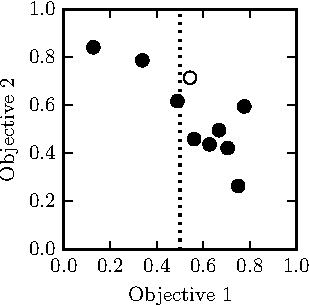
\includegraphics[scale=0.75]{econstraint}
        \caption{$\epsilon$-constraint with $\ell = 2$, $\epsilon_1 = 0.5$}
        \label{fig:experiments:setting:econstraint}
    \end{subfigure}
    \caption{Expected outcomes for optimal (white) and suboptimal (black) actions. The dotted line shows the preference function (left) and the $\epsilon_1$ constraint (right).}
\label{fig:experiments:setting}
\end{figure}

\begin{figure}[t]
    \centering
    \begin{subfigure}[b]{0.49\textwidth}
        \centering
        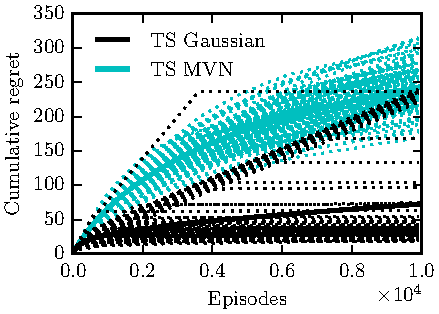
\includegraphics[scale=0.75]{bernoulli_linear}
        \caption{Multi-Bernoulli, linear}
    \end{subfigure}
    \begin{subfigure}[b]{0.49\textwidth}
        \centering
        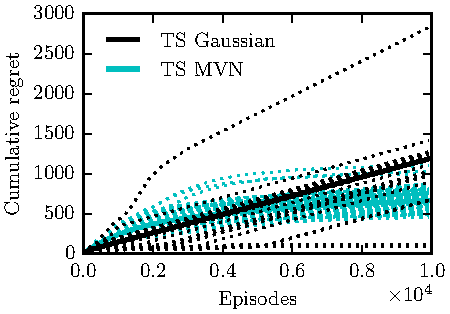
\includegraphics[scale=0.75]{bernoulli_econstraint}
        \caption{Multi-Bernoulli, $\epsilon$-constraint}
    \end{subfigure}

    \begin{subfigure}[b]{0.49\textwidth}
        \centering
        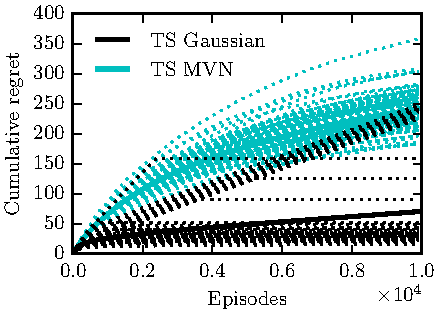
\includegraphics[scale=0.75]{normal_linear}
        \caption{Multivariate normal, linear}
    \end{subfigure}
    \begin{subfigure}[b]{0.49\textwidth}
        \centering
        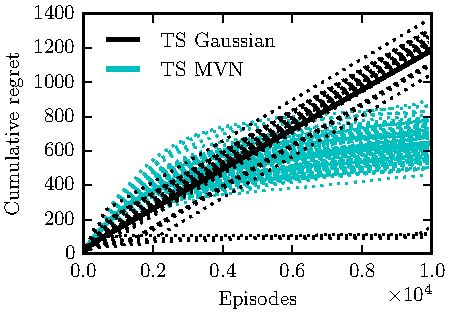
\includegraphics[scale=0.75]{normal_econstraint}
        \caption{Multivariate normal, $\epsilon$-constraint}
    \end{subfigure}
    \caption{Cumulative regret over episodes for tested outcome distributions and preference functions. Fat lines indicate the average over repetions and dotted lines indicate each individual repetition.}
\label{fig:experiments:results}
\end{figure}

Fig.~\ref{fig:experiments:results} shows the cumulative regret of TS from MVN priors and TS from Gaussian priors (in the traditional bandits formulation) for both outcome distributions and preference functions. We observe that the cumulative regret growth rate for TS from MVN priors appears to match the order of the provided theoretical bounds (Theorem~\ref{thm:mvn_ts}). Results also show that, though it might be appealing to address a multi-objective problem as a single-objective bandits problem, it is not a good idea. Consider the $\epsilon$-constraint preference function used in this experiment. It is evaluated as 0 if $z_1(t) < 0.5$, otherwise to $z_2(t)$. With multi-Bernoulli outcomes, for example, this means that $\Pr[f(\bsz(t)) = 1] = \mu_{a(t), 1} \mu_{a(t), 2}$. Given that, $\argmax_{a \in \cA} f(\bsmu_a) \neq \argmax_{a \in \cA} \Esp[f(\bsz(t)) | a(t) =a]$. Since the action considered as optimal in the single-objective formulation is not the same as the optimal action in the multi-objective problem, TS with Gaussian priors converges to the \emph{wrong} action, hence the linear regret.
